\documentclass{article}

\usepackage{amsmath}
\usepackage{graphicx}

\title{Report 4: Neural Network}
\author{Hoai Nam Le}

\begin{document}

\maketitle

\section{Network Architecture}

The neural network was implemented from scratch
using object oriented programming.

The implementation contains 3 classes:

\begin{itemize}
    \item Neuron
    \item Layer
    \item NeuralNetwork
\end{itemize}

The network architecture is read from a text file.

Example:

\begin{verbatim}
3
2
2
1
\end{verbatim}

Meaning:
\begin{itemize}
    \item 3 layers
    \item 2 input neurons
    \item 2 hidden neurons
    \item 1 output neuron
\end{itemize}

Each neuron contains:
\begin{itemize}
    \item weights
    \item bias
    \item sigmoid activation function
\end{itemize}

\section{Feedforward}

Each neuron computes a linear sum:

\[
z = \sum x_iw_i + b
\]

Then applies the sigmoid activation function:

\[
\sigma(z) = \frac{1}{1 + e^{-z}}
\]

The outputs of one layer become the inputs
of the next layer.

Feedforward is performed layer by layer until
the final output is obtained.

\section{XOR Experiment}

The XOR neural network was initialized using
the weights and biases from the lecture slides.

Hidden layer:

\[
[-10, -10],\ b = 15
\]

\[
[10, 10],\ b = -5
\]

Output layer:

\[
[10, 10],\ b = -15
\]

Inputs tested:

\begin{itemize}
    \item (0,0)
    \item (0,1)
    \item (1,0)
    \item (1,1)
\end{itemize}

\begin{figure}[h]
    \centering
    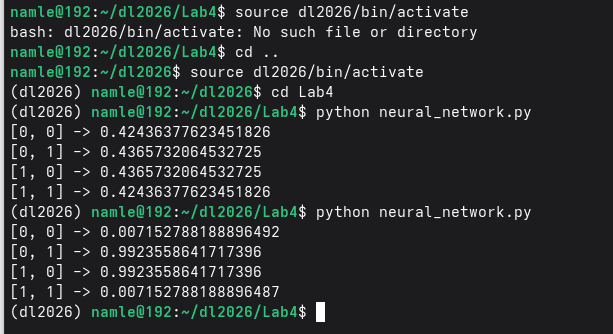
\includegraphics[width=0.5\textwidth]{result.png}
    \caption{Results of the XOR neural network}
\end{figure}
Results:

\begin{verbatim}
[0,0] -> 0.007
[0,1] -> 0.992
[1,0] -> 0.992
[1,1] -> 0.007
\end{verbatim}

The neural network successfully approximates
the XOR function.

\end{document}